% !TeX root = ../thuthesis-example.tex

\chapter{基于隐式神经表示的端到端拓扑优化方法}

\section{引言}
拓扑优化(Topology Optimization,TO)是一种计算设计方法论,旨在确定设计域内材料的最佳分布,以实现特定的性能目标,同时遵守给定的约束条件~\cite{sigmund2013}。在过去的三十年里,计算机技术和3D打印的进步推动了拓扑优化方法的重大进展。这些方法包括固体各向同性材料惩罚(SIMP)方法~\cite{bendsoe1999}、进化结构优化(ESO)方法~\cite{xie1993}、水平集方法(LSM)\cite{wang2003level}以及最近的可移动可变组件/空隙(MMC/MMV)方法\cite{guo2014doing,zhang2017explicit}。这些方法在结构表示方式上有所不同,但它们都是通过重复的物理响应分析和参数梯度信息来迭代地寻求最优的材料分布。拓扑优化的求解过程涉及反复的、计算密集型的有限元分析,以求解物理平衡方程。这种计算需求是这些方法效率低下的主要原因,从而阻碍了拓扑优化在实际应用场景中的推广。

为了提高效率,研究者们投入了大量精力,探索加速拓扑优化过程的有效方法~\cite{mukherjee2021}。这些方法采用了多种技术,如多网格求解器、模型缩减、高性能计算及其组合。近年来,人工智能(AI)在机械工程领域的影响显著增强。特别是,利用神经网络和深度学习技术解决拓扑优化问题的兴趣大幅增加~\cite{cang2019one,kollmann2020deep,nie2020optimization,chandrasekhar2021,hoang2022,woldseth2022}。在这些策略中,无迭代方法~\cite{li_cad_2019,behzadi_2021}引起了广泛关注。这些方法通过构建深度神经网络,直接从条件和问题配置中预测最优结构。通过这种直接设计方法实现近乎实时的拓扑优化,具有很大的吸引力。Sigmund等人在综述中指出了与直接设计方法相关的几个挑战性问题~\cite{woldseth2022}。首先,使用传统拓扑优化方法构建训练数据集计算成本高。其次,训练好的模型难以推广到未见样本。第三,常用的损失函数,如均方误差(MSE)或二元交叉熵(BCE),缺乏检测和防止结构断裂所需的敏感性。
本章提出了一种新颖的无迭代拓扑优化框架,称为IF-TOINR,旨在解决上述问题。

隐式神经表示(INR)最近受到了广泛关注\cite{deepsdf,nerf2020,xie2022,xu2023deformable}。INR利用神经网络生成离散信号场(如颜色、符号距离值或密度)的连续参数化表示。INR模型在各种挑战性领域的应用展示了其对输入数据变化的鲁棒性,以及对未见场景的良好泛化能力。受此启发,本文选择使用连续的\textit{符号距离场}(SDF)来表示结构。与基于密度的离散表示方法相比,这种表示方法提供了一种紧凑且平滑的表示,有效消除了棋盘现象。此外,INR的使用将设计过程与空间网格解耦,理论上能够以任何所需的精度获取结构。

IF-TOINR框架利用变分自编码器(VAE)从训练数据集中学习和重构最优结构的SDF。采用基于CNN的编码器将结构嵌入到低维潜在空间中。随后,基于MLP的解码器将设计域内特定点的坐标和来自已学习潜在空间的潜在向量作为输入,预测该点对应的SDF值,结合来自两个来源的信息。IF-TONIR包含一个名为\textit{物理网络}的子网络,负责从各种条件中提取特征,包括载荷、位移约束以及应力和应变场。将来自物理网络的特征向量作为条件码,指导VAE模型根据给定的问题配置生成结构。为了使网络识别设计域的形状,将设计域转换为其SDF表示。然后,将设计域的SDF值附加到每个点作为附加属性。这些点的坐标及其属性被输入到解码器中,以输出最优结构的SDF值。最终,通过提取其SDF的零水平集,获得最优结构。

损失函数的选择在训练神经网络中起着至关重要的作用。然而,经典的损失函数如均方误差(MSE)或二元交叉熵(BCE)仅关注局部离散信号误差,可能无法充分捕捉全局结构特征,如连通性。在本研究中,引入了一种基于计算拓扑学中持久同调技术的拓扑感知损失项~\cite{persistent2008}。该拓扑损失能够捕捉重构结构与真实结构(GT)之间的拓扑特征误差,如连通成分和孔洞的数量。实验结果验证了拓扑损失可以提高重构精度并减少结构断裂的发生。一旦模型训练完成,通过输入相关的设计域形状、问题配置和物理信息,即可直接推断出相应的最优结构。

\section{预备知识}\label{sec:preliminary}
\begin{figure*}[t!]
    \centering
    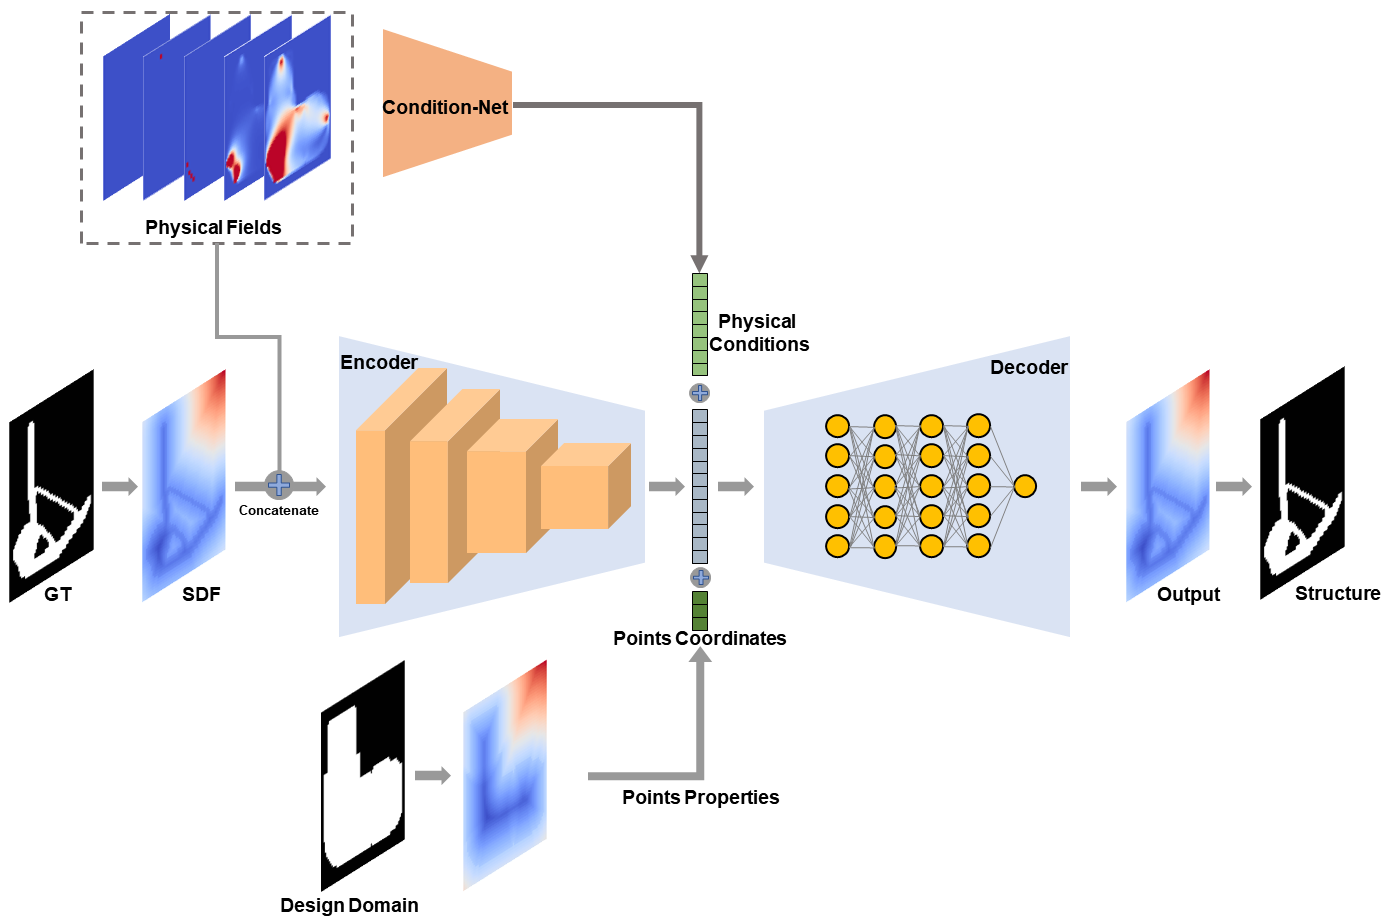
\includegraphics[width=0.95\textwidth]{./figures/TONIR/0-network-1.png}
    \caption{IF-TOINR算法整体框架图}
    \label{fig:network}
\end{figure*}

IF-TOINR算法原理框架如图~\ref{fig:network}所示,在介绍算法之前之前,章节~\ref{sec:preliminary}先介绍拓扑优化一般形式、结构隐式表示和持续同调技术的预备知识。

\subsection{拓扑优化一般形式}
\begin{figure}[b]
    \centering
    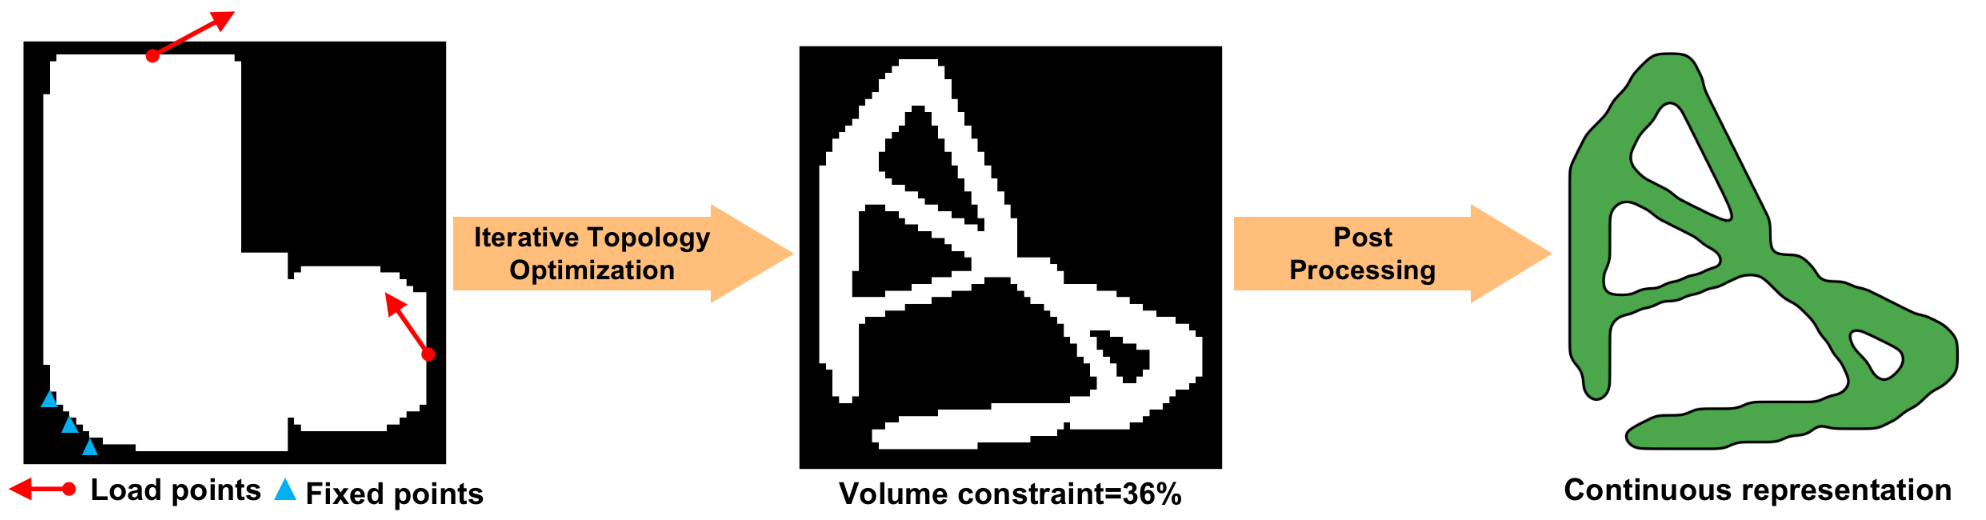
\includegraphics[width=0.9\textwidth]{./figures/TONIR/1-TO.png}
    \caption{传统拓扑优化的一般流程}
    \label{fig:TO}
\end{figure}
拓扑优化旨在优化指定域内的材料分布,以满足特定的目标和约束。本章算法在著名的最小结构柔度问题上评估了所提出的算法。值得注意的是,给定合适的数据集,本方法可以扩展到具有不同目标和约束的拓扑优化问题,如应力相关问题~\cite{le2010stress}或热传导问题~\cite{takezawa2014}。具体来说,本文考虑在体积约束下的二维最小柔度问题。如图~\ref{fig:TO} (左)所示,当在给定域上施加特定载荷以及附加的边界位移约束时,会引出以下问题的公式化:
\begin{subequations}\label{eq:opti_problem}
    \begin{align}
        \min_{\Theta}~
         & C(\Theta)=\int_{\Omega_\Theta} \mathbf{f}\cdot\mathbf{u}~\mathrm{d}\sigma+\int_{\Gamma_T} \mathbf{t}\cdot\mathbf{u}~\mathrm{d}s,                              \\
        \text{s.t.:}~
         & \int_{\Omega_\Theta}\mathbb{E}:\varepsilon(\mathbf{u}):\varepsilon(\mathbf{v})~\mathrm{d}\sigma = \int_{\Omega_\Theta}\mathbf{f}\cdot\mathbf{v}~\mathrm{d}\sigma+\int_{\Gamma_T}\mathbf{t}\cdot\mathbf{v}~\mathrm{d}s,~\forall \mathbf{v}\in\mathcal{U}_{ad}, \\
         & \mathbf{u}=\mathbf{\overline{u}},~\text{on}~\Gamma_u,                                                                                                         \\
         & \int_{\Omega_\Theta}1~\mathrm{d}\sigma\leq\overline{V},
    \end{align}
\end{subequations}
其中,$C$ 是结构柔度,衡量总的结构应变能,较低的 $C$ 值表示结构刚度更大。$\Omega_\Theta$ 是结构所占据的区域,$\Theta$ 是控制结构几何和拓扑的优化变量。$\mathbf{f}$ 是外力,$\mathbf{t}$ 是定义在 Neumann 边界上的牵引力,$\mathbf{u}$ 是位移场,$\mathbf{v}$ 是定义在 $\Omega_\Theta$ 上的相应测试函数,$\mathcal{U}_{ad}$ 是运动学上可接受的位移场空间。$\varepsilon$ 是二阶线性应变张量,$\mathbb{E}$ 是由杨氏模量和泊松比决定的四阶各向同性弹性张量,$\overline{\mathbf{u}}$ 是在 Dirichlet 边界 $\Gamma_u$ 上的规定位移,$\overline{V}$ 是给定的体积约束。在传统的 SIMP 方法中,$\Theta$ 表示离散元素的密度。通过迭代优化算法获得最优的密度分布,如图~\ref{fig:TO} (中) 所示。随后,进行一系列后处理操作以获得连续的最优结构表示,如图~\ref{fig:TO} (右) 所示。在该算法中,SDF 的连续性使表示的调整变得简单,能够根据需要细化结构特征或引入平滑操作。


\subsection{结构的隐式表示}
\begin{figure}[b]
    \centering
    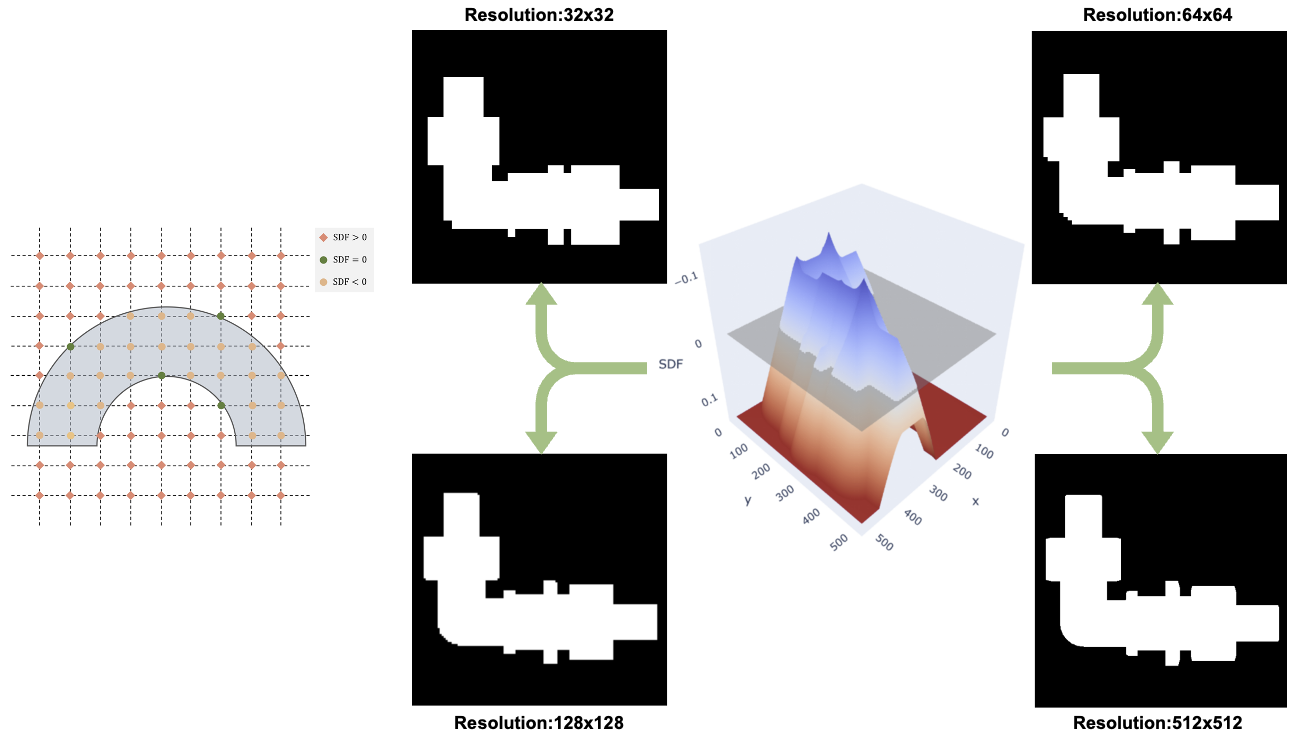
\includegraphics[width=1.0\textwidth]{./figures/TONIR/2-SDF.png}
    \caption{基于SDF的结构表示}
    \label{fig:SDF}
\end{figure}
符号距离场(SDF)是一种广泛使用的几何模型表示方法,它为空间中的每个点分配一个符号距离值,表示该点与结构边界上最近点之间的距离。距离的符号表明该点位于结构的内部或外部,如图~\ref{fig:SDF} (a) 所示。在结构占据的区域内,如图~\ref{fig:SDF} (b) 所示,可以定义一个连续的符号距离函数 $\phi_\Theta(\textbf{x})$,其满足以下条件:
\begin{equation}
    \phi^{SDF}_\Theta(\mathbf{x})
    \begin{cases}
        >0, & \text{if $\mathbf{x}$ is inside},          \\
        =0, & \text{if $\mathbf{x}$ is on the boundary}, \\
        <0, & \text{if $\mathbf{x}$ is outside}.
    \end{cases}
\end{equation}
通过提取 $\phi_\Theta$ 的零水平集,可以轻松获得结构的边界。本章算法利用神经网络拟合结构的 SDF,网络参数记为 $\Theta$。这种隐式表示方法的主要优点是与空间网格解耦,输入设计域内任意点的坐标,即可获得相应的 SDF 值,无需依赖预定义的空间网格。理论上,这使得可以在任何所需分辨率下获取结构(如图~\ref{fig:SDF} (c) 所示)。然而,需要注意的是,结构细节的复杂性取决于所使用神经网络的表达能力,更复杂的神经网络能够捕捉到更复杂的结构细节。鉴于训练数据集来源于SIMP方法,该方法生成结构的密度场,因此需要在SDF和密度场之间建立相互转换。通过经典的距离变换方法~\cite{maurer2003linear},从结构的密度场导出SDF。一旦获得结构的SDF,即可将其转换为密度场,具体步骤如下:
\begin{equation}
    \phi^{D}(\phi^{SDF}(\mathbf{x}))=
    \begin{cases}
        0, & \text{if}\quad \phi^{SDF}(\mathbf{x}) > 0,\\
        1, & \text{if}\quad \phi^{SDF}(\mathbf{x})\leq 0.
    \end{cases}
\end{equation}



\subsection{基于立方复形的持续同调分析}
\label{sec:PH}
拓扑数据分析(TDA)是一种创新方法,结合了拓扑学、几何学和数据科学,以揭示复杂数据集中有意义的模式和结构。通过关注数据的固有形状和连接性,TDA 提供了宝贵的见解和对数据内部关系的深入理解。单纯复形~\cite{rotman2013} 常用于离散数据空间,表示数据点之间的连接关系。本文使用立方复形来分析结构的隐式神经表示的拓扑特征。由于结构使用符号距离场表示,立方复形提供了一个有效的框架,用于提取和分析这些表示中编码的潜在拓扑信息。

\begin{definition}[\textbf{立方复形}]
    一个立方复形 $\mathcal{C}$ 是一组有限的 $n$ 维立方体,形式为 $[a_1, b_1] \times \cdots \times [a_n, b_n]$,其中 $a_i, b_i \in \mathbb{R}$ 且 $a_i \leq b_i$,并满足以下条件:

    \begin{enumerate}
        \item 如果一个立方体 $c \in \mathcal{C}$,那么 $c$ 的所有面也在 $\mathcal{C}$ 中。
        \item 如果两个立方体 $c_1, c_2 \in \mathcal{C}$ 有非空交集,那么它们的交集要么是 $c_1$ 和 $c_2$ 的一个面,要么是 $\mathcal{C}$ 中的一个立方体。
    \end{enumerate}

\end{definition}

直观地说,在基于二维数据的立方复形中,基本元素包括点(0维立方体)、线段(1维立方体)和正方形(2维立方体)。图~\ref{fig:ph-illu}(a) 展示了使用离散元素对结构进行二值化表示。在这种表示中,密度值等于1的元素(实心元素)组合形成立方复形 $\mathcal{C}_s$,可以计算 $\mathcal{C}_s$ 的拓扑特征,即 \textbf{\textit{Betti 数}}。Betti 数反映了结构中连通分量的数量(0维 Betti 数 $\beta_0$)和孔洞的数量(1维 Betti 数 $\beta_1$)。然而,Betti 数是离散的拓扑特征,不可微,不能直接用于网络训练。为了解决这个问题,使用持久同调方法提取结构的拓扑特征。

持久同调~\cite{edelsbrunner2000} 是一种强大的数学工具,用于计算和分析嵌套单纯复形中的多维拓扑特征。它可以跟踪超水平集滤波中所有复形上的拓扑特征演变,如定义~\ref{def:filtration} 所述。根据研究问题,有多种定义滤波的方法。在本文算法中,将结构的SDF(图~\ref{fig:ph-illu}(b))作为分配给 $\mathcal{C}_s$ 的滤波函数。然后,定义一个连续特征度量,即 \textbf{\textit{持久性}},用于分析数据的多维拓扑特征,如定义~\ref{def:persistence} 所述。可以将拓扑特征的出生值、死亡值和持久性编码在一个 \textbf{\textit{持久性图}}(PD)中,如图~\ref{fig:ph-illu}(c) 所示。持久性图作为一个多维形状描述符,捕捉结构的所有拓扑特征。

\begin{definition}[\textbf{超水平集滤波}]
    \label{def:filtration}
    定义一个 滤波函数 $f:\mathcal{C}_s\rightarrow\mathbb{R}$,它为 $\mathcal{C}_s$ 中的每个元素分配一个实数值。函数 $f$ 的超水平集滤波是一个嵌套的复形序列 $\emptyset\subseteq\mathcal{C}_0\subseteq\mathcal{C}_1\subseteq\cdots\subseteq\mathcal{C}_n=\mathcal{C}_s$,其中 $\mathcal{C}_i={c\in\mathcal{C}_s|f(c)\leq\alpha_i}$,且 $\alpha_0\leq\alpha_1\leq\cdots\leq\alpha_n$。
\end{definition}

\begin{definition}[\textbf{持久性}]
    \label{def:persistence}
    对于一个拓扑特征 $\beta_k$,其 \textit{持久性} 定义为该特征的出生值与死亡值之间的差,即 $\text{pers}(\beta_k)=|\alpha_i-\alpha_j|$,其中出生值 $\alpha_i$ 和死亡值 $\alpha_j$ 分别对应于该特征被创建和消失时的滤波值。持久对 $(\alpha_i, \alpha_j)$ 也描述了拓扑特征。特别地,$(\alpha_i, +\infty)$ 反映了一个在 $\alpha_i$ 处出生并持续到滤波结束的特征。
\end{definition}

\begin{figure}[htbp]
    \centering
    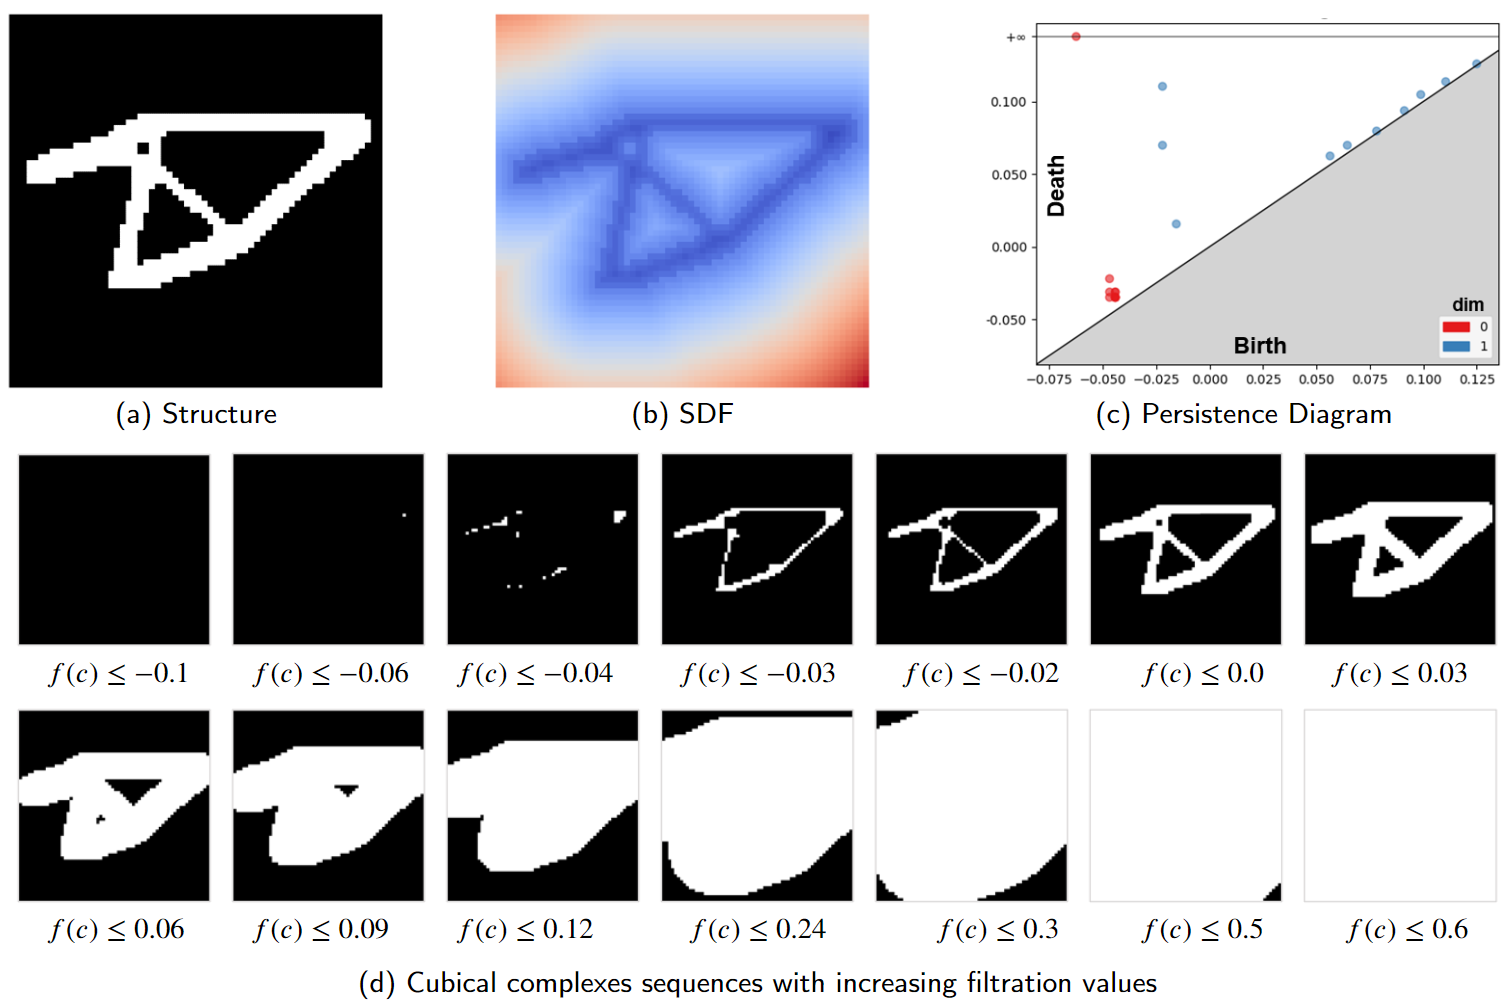
\includegraphics[width=0.95\textwidth]{./figures/TONIR/topo-PD-illu}
    \caption{基于持续同调技术的拓扑特征表示示意图}
    \label{fig:ph-illu}
\end{figure}

\section{研究方法}
本算法采用SIMP方法生成二维数据集,得到在特定条件下(包括载荷、位移约束和体积约束)最小化结构柔度的最优结构(称为真实值,GT)。IF-TONIR的关键思想是利用变分自编码器(VAE)重建最优结构。通过训练,网络捕捉结构特征并将其编码到低维潜在空间中。然后,从这个潜在空间生成相应的最优结构,同时考虑边界信息和设计域形状作为条件。具体而言,使用物理网络从边界条件和物理场中提取特征。这个特征向量作为条件码,引导网络根据给定问题配置生成结构。通过将点坐标及其与设计域形状相关的属性输入解码器,网络可以有效识别材料可分布的设计区域。

\subsection{数据集}
将训练良好的模型推广到任意设计域和约束条件可能具有挑战性,即使是形状相似但略有差异的设计域,在传统拓扑优化方法中通常也需要新的迭代优化过程。为了解决这一问题,准备了一个数据集,将具有相似特征的设计域分类为组,如图~\ref{fig:datasets}(a) 所示。在这个由该组设计域生成的最优结构组成的数据集上训练IF-TONIR。因此,在处理形状相似的设计域时,网络可以直接预测相应的最优结构。

\begin{figure}[t]
    \centering
    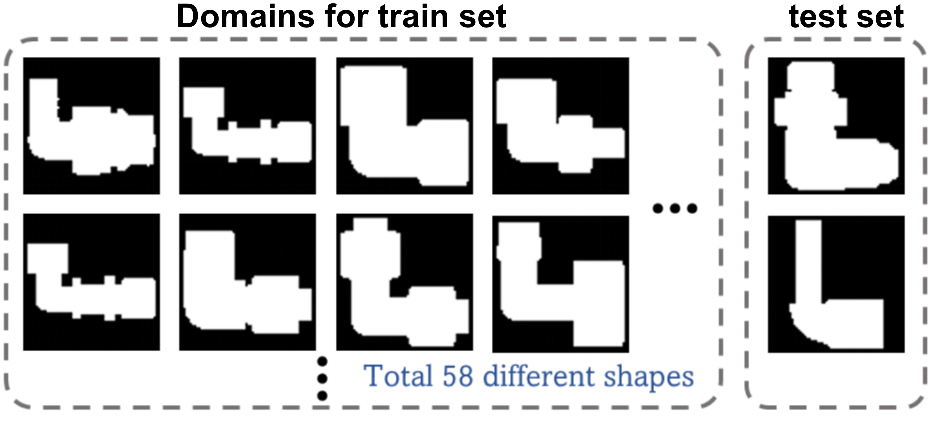
\includegraphics[width=0.6\textwidth]{./figures/TONIR/domains_set.png}
    \hspace{0.2cm}
    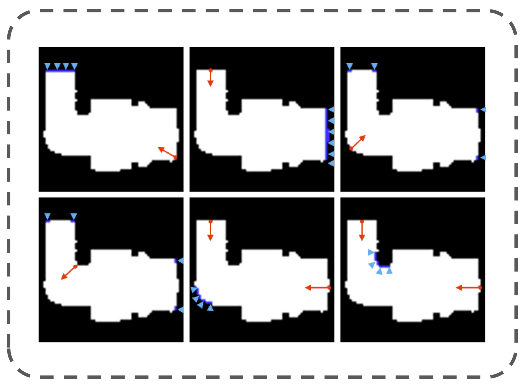
\includegraphics[width=0.35\textwidth]{./figures/TONIR/bd_types.png}
    % \includegraphics[width=0.3\textwidth]{./figs/op_structures_set.png}
    \\
    \makebox[0.6\textwidth]{\small (a) 具有相似形状的一类设计域.}
    \hspace{0.2cm}
    \makebox[0.35\textwidth]{\small (b)六种边界条件}
    % \makebox[0.3\textwidth]{\small (c) Optimal structures }
    \caption{数据集准备}
    \label{fig:datasets}
\end{figure}

此外,考虑到实际应用中,尽管尺寸不同,但具有相同功能的工业部件通常具有相似的载荷情况,因此无需要求网络推广到任意载荷条件。因而,为每个形状设计域设置了六种边界条件(图~\ref{fig:datasets}(b))。每个边界条件包括不同的载荷方向和体积约束。IF-TONIR的潜在应用场景是,对于需要优化的形状相似的部件,训练于先前最优结构的网络可以直接生成优化解,而无需迭代。
文献~\cite{ferrari2020} 提供了一个紧凑且高效的SIMP Matlab实现,用于生成相应的最优结构作为真实值。生成训练数据集的具体参数详见表~\ref{tab:settings}。在准备数据集时,固定每个设计域类别中形状的材料属性。在实验设置中,杨氏模量和泊松比分别设为1.0和0.2。将体积约束和力的方向作为每个优化问题的变量,使用传统方法~\cite{ferrari2020} 迭代获得优化结果,这些结果作为训练的真实值。本工作提供了一种连续梯度惩罚方案,以减少SIMP方法中的棋盘现象,从而优化具有清晰边界的结构。此外,与固定惩罚系数相比,该方案可以生成柔度更低的结构。因此,采用文章中提供的SIMP惩罚设置参数${50,3,25,0.25}$来生成优化问题的优化结构。

\begin{table}[htbp]
    \centering
    \parbox{0.45\textwidth}{
        \caption{用于生成数据集的参数设置}
        \label{tab:settings}
        \centering
        \resizebox{0.4\textwidth}{!}{
            \scriptsize
            \begin{tabular}{cc}

                \toprule
                参数                                                                   & 设置           \\
                \midrule
                体积约束                                                           & $[0.3:0.02:0.5]$   \\
                施力方向                                                               & $[0:\pi/6:\pi]$    \\
                分辨率                                                                   & $64\times 64$      \\
                SIMP 惩罚因子 & $\{50,3,25,0.25\}$ \\
                SIMP 滤波半径                                                          & 10                 \\
                杨氏模量                                                                & 1.0                \\
                泊松比                                                              & 0.2                \\
                \bottomrule
            \end{tabular}
        }}
    \vspace*{\baselineskip}
    \parbox{0.5\textwidth}{\centering \includegraphics[width=0.5\textwidth]{./figures/TONIR/op_structures_set.png}}
\end{table}

观察到,在相应边界条件下,原始设计域的物理响应分析结果与最优结构之间存在很强的相关性。因此,除了SDF表示和边界条件外,还计算了原始结构在载荷和位移约束下的应力场和应变能场。这些额外的物理场作为训练过程中的补充信息,在之前的工作中(如TopologyGAN~\cite{topologygan2021} 和 TopoDiff~\cite{maze2022})已被验证有效。

\subsection{网络结构}
网络架构主要包括两个部分,如图~\ref{fig:network} 所示,包含一个基于变分自编码器的最优结构重建网络,以及一个负责将边界条件和物理场编码为条件码的物理网络。

\subsubsection{网络输入}
在数据集中,原始二维最优结构表示为分辨率为64$\times$64的二值图像,其中“1”(白色)表示实心元素,“0”(黑色)表示空心元素。将结构的SDF $\{\mathbf{s}^s_i\}_{i=1}^N$ 计算为VAE网络的输入(如图~\ref{fig:input} (a)),其中$N$为样本总数。由于VAE是一种自监督学习方法,SDF $\mathbf{s}^s_i$ 也作为网络回归输出的真实值(GT)。此外,设计域的SDF $\{\mathbf{s}^d_i\}_{i=1}^N$ 作为属性附加到点上,用于识别设计域的形状(如图~\ref{fig:input} (b))。

如图~\ref{fig:input} (c)所示,载荷和位移约束表示为二维稀疏矩阵。在载荷矩阵中(包括$x$方向和$y$方向),每个元素的值为力值。位移约束使用相同大小的矩阵表示,值为1的元素表示相应元素在$x$和$y$方向上的位移约束为0,而值为0的元素表示无约束元素。补充的物理信息包括在特定载荷和位移约束下原始结构的应力场和应变场,这些信息通过SolidsPy~\cite{solidspy}计算得到。通过整合这五个场,获得物理信息数据样本$\{\mathbf{s}^{phy}_i\}_{i=1}^N$。

\begin{figure}[htbp]
    \centering
    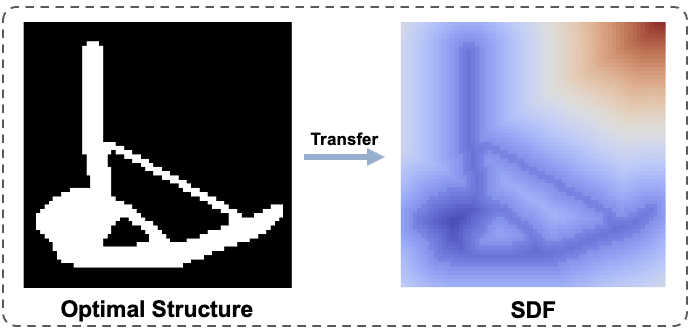
\includegraphics[width=0.4\textwidth]{./figures/TONIR/input-a.png}
    \hspace{0.08\textwidth}
    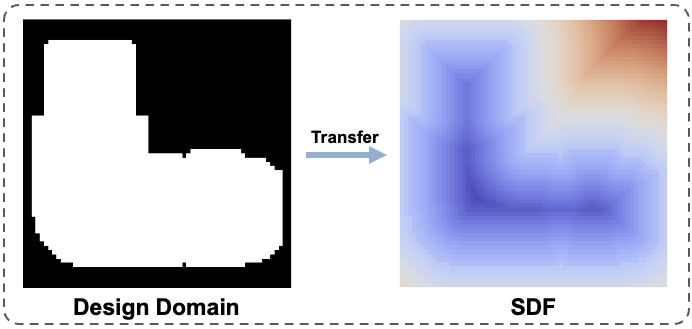
\includegraphics[width=0.4\textwidth]{./figures/TONIR/input-b.png}
    \\
    \makebox[0.4\textwidth]{(a) 转换最优结构到SDF}
    \hspace{0.08\textwidth}
    \makebox[0.4\textwidth]{(b) 转换设计域到 SDF.}
    \\
    \vspace{0.1 cm}
    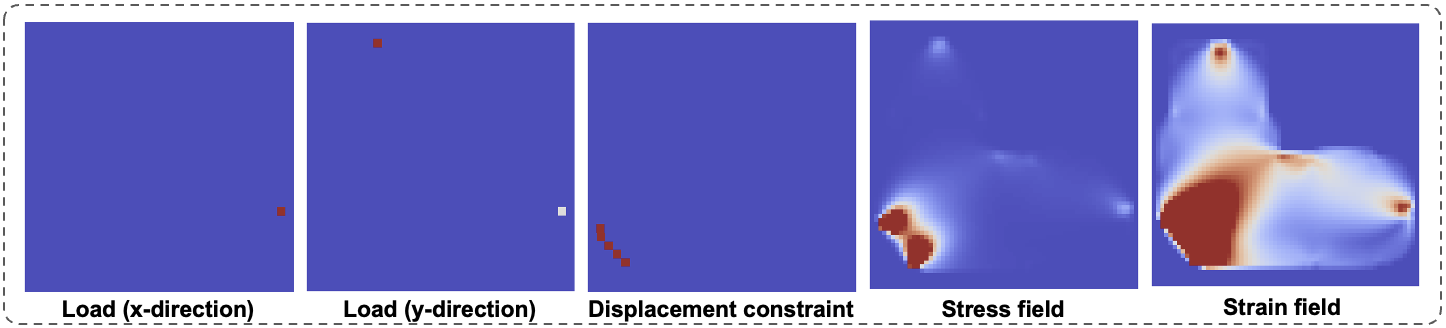
\includegraphics[width=0.9\textwidth]{./figures/TONIR/input-c.png}
    \\
    \makebox[0.9\textwidth]{(c) 边界条件和物理信息}
    \caption{网络输入数据信息构成}
    \label{fig:input}
\end{figure}

\subsubsection{用于结构重建的VAE}
IF-TONIR的主要目标之一是对输入的最优结构进行先验学习和隐式重建。为此,采用了变分自编码器(VAE)网络,这是一种广泛使用的生成模型。VAE网络由编码器和解码器组成。在该方法中,使用ResNet18架构作为编码器。ResNet18~\cite{he2016deep}是一种知名的卷积神经网络架构,在各种图像相关任务中表现出色。编码器通过一系列二维卷积层处理最优结构的输入SDF,提取特征并将其映射到低维潜在空间。此外,还将条件信息$\{\mathbf{s}^{phy}_i\}_{i=1}^N$输入到编码器中。编码器$\phi^E$的目的是学习潜在编码$\mathbf{z}_i$的分布,该编码能够重建输入数据$\mathbf{s}^s_i$。通常,假设潜在编码$\mathbf{z}_i$遵循高斯分布,
\begin{equation}
    q_{\phi^E}(\mathbf{z}_i|\mathbf{s}^s_i,\mathbf{s}^{phy}_i) = \mathcal{N}(\mu_{\phi^E}(\mathbf{s}^s_i,\mathbf{s}^{phy}_i),\sigma_{\phi^E}(\mathbf{s}^s_i,\mathbf{s}^{phy}_i)),
\end{equation}
其中,$\mu_{\phi^E}(\mathbf{s}^s_i)$和$\sigma_{\phi^E}(\mathbf{s}^s_i)$是由编码器$\phi^E$参数化的潜在编码的均值和方差。然后,采用重新参数化技巧~\cite{kingma2019introduction}将潜在编码$\mathbf{z}_i$表示为:
\begin{equation}
    \mathbf{z}_i = \mu_{\phi^E}(\mathbf{s}^s_i,\mathbf{s}^{phy}_i) + \sigma_{\phi^E}(\mathbf{s}^s_i,\mathbf{s}^{phy}_i) \odot \epsilon,
\end{equation}
其中,$\epsilon$是从标准高斯分布中采样的随机变量,$\odot$是元素逐个相乘。编码之后,采用基于多层感知器(MLP)的解码器$\phi^D$对潜在编码$\mathbf{z}_i$进行解码,并重建最优结构的SDF。在设计域内采样点,并将这些点的坐标输入到解码器中。解码器返回每个点的符号距离值。通过这种方式,解码器有效地充当结构的符号距离函数。在训练过程中,在设计域内均匀采样$64\times 64$个点$\{\mathbf{p}_k\}_{k=1}^M$。通过最小化解码器输出的SDF $\hat{\mathbf{s}}^s_i$与GT输入之间的重建误差来训练网络。

以下列出IF-TONIR的网络架构细节,采用浅层卷积神经网络(如表~\ref{tab:arch-cnn}所示)从边界设置和物理场中提取特征作为条件。对于VAE,使用ResNet18~\cite{rw2019timm}作为编码器,使用MLP作为解码器(如表~\ref{tab:arch-mlp}所示)。
\begin{table}
    \small
    \centering
    \begin{minipage}[b]{0.45\linewidth}
    \resizebox{0.8\textwidth}{!}{
    \begin{tabular}[t]{*{5}{c}}
        \hline
        \multicolumn{5}{c}{\textbf{CNN}} \\
        \hline
        \textbf{网络层} & \textbf{卷积核尺寸} & \textbf{卷积步长} & \textbf{卷积补丁} & \textbf{通道数}  \\
        \hline 
        2D Conv   & $3\times 3$     & $1$ & $1$    & $5 \rightarrow 64$  \\
        \multicolumn{5}{l}{Batch Norm}\\
        \multicolumn{5}{l}{LeakyReLU} \\
        Max Pool   & $2$     & $1$ &$1$   & $64 \rightarrow 64$  \\
        \hline
        2D Conv   & $3\times 3$     & $1$  &$1$  & $64 \rightarrow 64$   \\
        \multicolumn{5}{l}{Batch Norm}\\
        \multicolumn{5}{l}{LeakyReLU} \\
        Max Pool   & $2$     & $1$  &$1$  & $64 \rightarrow 64$  \\
        \hline
        2D Conv   & $3\times 3$     & $1$  &$1$  & $64 \rightarrow 32$   \\
        \multicolumn{5}{l}{Batch Norm}\\
        \multicolumn{5}{l}{LeakyReLU} \\
        Max Pool   & $2$     & $1$  &$1$  & $32 \rightarrow 32$  \\
        \hline
        2D Conv   & $3\times 3$     & $1$  &$1$  & $32 \rightarrow 32$   \\
        \multicolumn{5}{l}{Batch Norm}\\
        \multicolumn{5}{l}{LeakyReLU} \\
        Max Pool   & $2$     & $1$  &$1$  & $32 \rightarrow 32$  \\
        \hline
        2D Conv   & $3\times 3$     & $1$  &$1$  & $32 \rightarrow 32$   \\
        \multicolumn{5}{l}{Batch Norm}\\
        \multicolumn{5}{l}{LeakyReLU} \\
        Max Pool   & $2$     & $1$ &$1$   & $32 \rightarrow 32$  \\
        \hline
        \multicolumn{5}{c}{Output: $1\times 128$}\\
        \hline
        % % \rowcolor{gray!25}\multicolumn{4}{|c|}{\textbf{Output: 128\times 1}} \\
        % \hline
    \end{tabular}
     }
    \caption{用于提取物理场特征的CNN网络架构}
    \label{tab:arch-cnn}
    \end{minipage}
    \begin{minipage}[b]{0.45\linewidth}
    \small
    \resizebox{1.0\textwidth}{!}{
        \begin{tabular}[t]{*{4}{c}}
        \hline
        \multicolumn{4}{c}{\textbf{基于MLP的解码器}} \\
        \hline
        \textbf{网络层} & \textbf{输入维度} & \textbf{输出维度} & \textbf{丢弃率}  \\
        \hline 
        Fully Connected   & $dim_{z}+dim_{c}+dim_{p}$     & 512    & 0.0   \\
        Fully Connected   & 512     & 512    & 0.0   \\
        \multicolumn{4}{l}{Batch Norm}\\
        Fully Connected   & 512     & 512    & 0.1   \\
        \multicolumn{4}{l}{Batch Norm}\\
        Fully Connected   & 512     & 512    & 0.0   \\
        \multicolumn{4}{l}{Batch Norm}\\
        Fully Connected   & 512     & 512    & 0.1 \\
        \multicolumn{4}{l}{Batch Norm}\\
        Fully Connected   & 512+$dim_{p}$     & 512    & 0.0   \\
        \multicolumn{4}{l}{Batch Norm}\\
        Fully Connected   & 512     & 512    & 0.0   \\
        \multicolumn{4}{l}{Batch Norm}\\
        Fully Connected   & 512 & 512 & 0.1 \\
        \multicolumn{4}{l}{Batch Norm}\\
        Fully Connected   & 512+$dim_{p}$     & 512   & 0.0 \\
        \multicolumn{4}{l}{Batch Norm}\\
        Fully Connected   & 512 & 1 & 0.0\\
        \hline
        \multicolumn{4}{l}{tanh}\\
        \hline
    \end{tabular}
    }
    \caption{用于生成最优结构的解码器}
    \label{tab:arch-mlp}
    \end{minipage}
\end{table}

\subsubsection{条件信息输入}
为了使网络能够在各种设计域形状和边界条件下生成结构,必须将条件信息纳入网络中。为此,引入了先验概率分布$p(\mathbf{s}^s_i|\mathbf{c})$,其中$\mathbf{c}$表示条件信息。条件信息包括设计域形状、载荷、位移约束和体积约束等。

边界设置包括五个二维张量,分别是$x$和$y$方向的载荷矩阵、位移约束矩阵、应力场和应变场。采用浅层卷积神经网络(CNN)有效表示和编码这些边界信息作为条件。CNN网络以边界张量$\mathbf{s}_I^{phy}$为输入,通过一系列卷积层处理,捕捉相关特征和模式。这使得物理网络能够生成包含边界条件关键信息的潜在编码$\mathbf{c}^{phy}_i$。通过将边界条件编码为潜在编码,使网络在生成过程中能够有效利用这些信息,确保生成的结构与指定的边界条件一致。

由于解码器基于设计域内输入点$\mathbf{p}_k=(x_k,y_k)\in\Omega$的坐标输出SDF值,可以将形状信息和体积约束作为附加属性添加到该点。属性$\mathbf{s}^d_i(\mathbf{p}_k)$帮助网络识别设计域的形状,从而确定材料分布的边界。将体积约束$v_i$作为属性附加到每个点上,可以看作是表示该点处材料存在或不存在的概率密度分布。因此,将与每个点相关的向量$\mathbf{c}_k^{pro}=(x_k, y_k, \mathbf{s}^d_i(\mathbf{p}), v_i)$输入到解码器中。这使得网络在生成SDF值时能够考虑设计域形状和体积约束。Rahaman等人~\cite{rahaman2019}证明了深度神经网络倾向于学习低频函数,这可能限制其准确拟合高频变化数据的能力。借鉴NeRF~\cite{nerf2020}的灵感,使用编码函数$\gamma(t)$将点属性$t\in\mathbb{R}$映射到高维空间$\mathbb{R}^{2L}$:
\begin{equation}
    \gamma(t)=(\sin(2^0\pi t),\cos(2^0\pi t),\sin(2^1\pi t),\cos(2^1\pi t), \cdots, \sin(2^{L-1}\pi t),\cos(2^{L-1}\pi t)),
    \label{eq:pe}
\end{equation}
其中,$L$是一个超参数,决定了编码函数的频率。在实验中,设定$L=4$用于编码输入点$\mathbf{p}_k=(x_k,y_k)$的坐标,$L=6$用于编码$\mathbf{s}^d_i(\mathbf{p}_k)$,$L=10$用于编码体积约束。此外,还可以将载荷和位移约束作为属性添加到点上,进一步增强网络识别边界条件的能力。

综上所述,将最优结构的潜在编码$\mathbf{z}_i$、条件编码$\mathbf{c}^{phy}_i$和点属性$\mathbf{c}_k^{pro}$进行连接。然后将组合向量输入解码器进行结构生成。通过整合这些组件,网络能够利用潜在空间、条件信息和点属性,生成满足设计域形状和条件的最优结构。

\subsection{损失函数和评估指标}
与经典的变分自编码器(VAE)类似,IF-TONIR在训练过程中使用包含重构损失和KL散度损失的损失函数。然而,为了提高结构重构的准确性,除了传统的几何损失外,还引入了拓扑损失。该拓扑损失旨在确保生成的结构具有与GT结构相同的拓扑。

\subsubsection{几何损失}
几何损失衡量网络预测的SDF值$\hat{\mathbf{s}}^s_i$与结构的GT SDF值$\mathbf{s}^s_i$之间的回归误差。值得注意的是,结构的形状主要由其边界决定,而非边界点的值则不太重要。为了优先保证边界附近点的准确性,采用了在公式~\eqref{eq:cl1-loss}中定义的夹紧$L_1$损失函数~\cite{park2019deepsdf},这使得IF-TONIR能够有效捕捉结构细节并保持所需的形状特征,
\begin{equation}
    \label{eq:cl1-loss}
    \mathcal{L}_{clamp}(\hat{\mathbf{s}}^s_i,\mathbf{s}_i^s)=\frac{1}{M}\sum_{k=1}^M\lvert~\chi (\hat{\mathbf{s}}^s_i(\mathbf{p}_k),\tau)-\chi (\mathbf{s}_i^s(\mathbf{p}_k),\tau)~\rvert,
\end{equation}
其中, $M$是设计域采样点总数, $\chi (x,\tau)=\min(\tau,\max(-\tau,x))$.

为了对输出结构施加体积约束,加入了一个体积损失项,该损失项量化了预测结构与目标结构在体积上的差异。通过以下积分方程从结构的SDF表示中计算其体积~\cite{van2012explicit}:
\begin{equation}
    V(\mathbf{s})=\int_{\Omega}H(-\mathbf{s}(\mathbf{p}))\,\,\mathrm{d}A,
\end{equation}
其中,$\Omega$是整个设计域,$\mathrm{d}A$是面积元素,$H(\cdot)$是Heaviside函数,
\begin{equation}
    H(x)=
    \begin{cases}1 ,\,\,                                                           & \textrm{if}\,\,  x< -\eta,            \\
             \frac{3}{4}(\frac{x}{\eta}-\frac{x^3}{3\eta^3})+\frac{1}{2}, \,\, & \textrm{if}\,\,  -\eta\leq x\leq\eta, \\
             0,\,\,                                                            & \textrm{if}\,\,  x>\eta.
    \end{cases}
\end{equation}
然后定义体积损失如下:
\begin{equation}
    \label{eq:vol-loss}
    \mathcal{L}_{vol}(\hat{\mathbf{s}}^s_i,\mathbf{s}_i^s)=\lvert~V(\hat{\mathbf{s}}^s_i)-V(\mathbf{s}_i^s)~\rvert /V(\mathbf{s}^s_i).
\end{equation}
综上,几何损失就是 clamped $L_1$损失, MSE损失和体积损失的和:
\begin{equation}
    \label{eq:geo-loss}
    \mathcal{L}_{geo}(\hat{\mathbf{s}}^s_i,\mathbf{s}_i^s)=\mathcal{L}_{clamp}(\hat{\mathbf{s}}^s_i,\mathbf{s}_i^s)+\mathcal{L}_{vol}(\hat{\mathbf{s}}^s_i,\mathbf{s}_i^s).
\end{equation}
在实验中,本算法设置 $\tau=0.05, \eta=0.02$。

\subsubsection{拓扑损失}
几何损失关注局部信息,而拓扑损失捕捉全局结构特征。如图~\ref{fig:loss_compare}(b)所示,小的结构缺陷可能导致结构断裂,从而显著降低结构的顺应性。然而,这些错误在几何损失中可能只会导致小的数值。通过引入拓扑损失,IF-TONIR能够有效检测和衡量微小的结构断裂。
\begin{figure}[htbp]
    \centering
    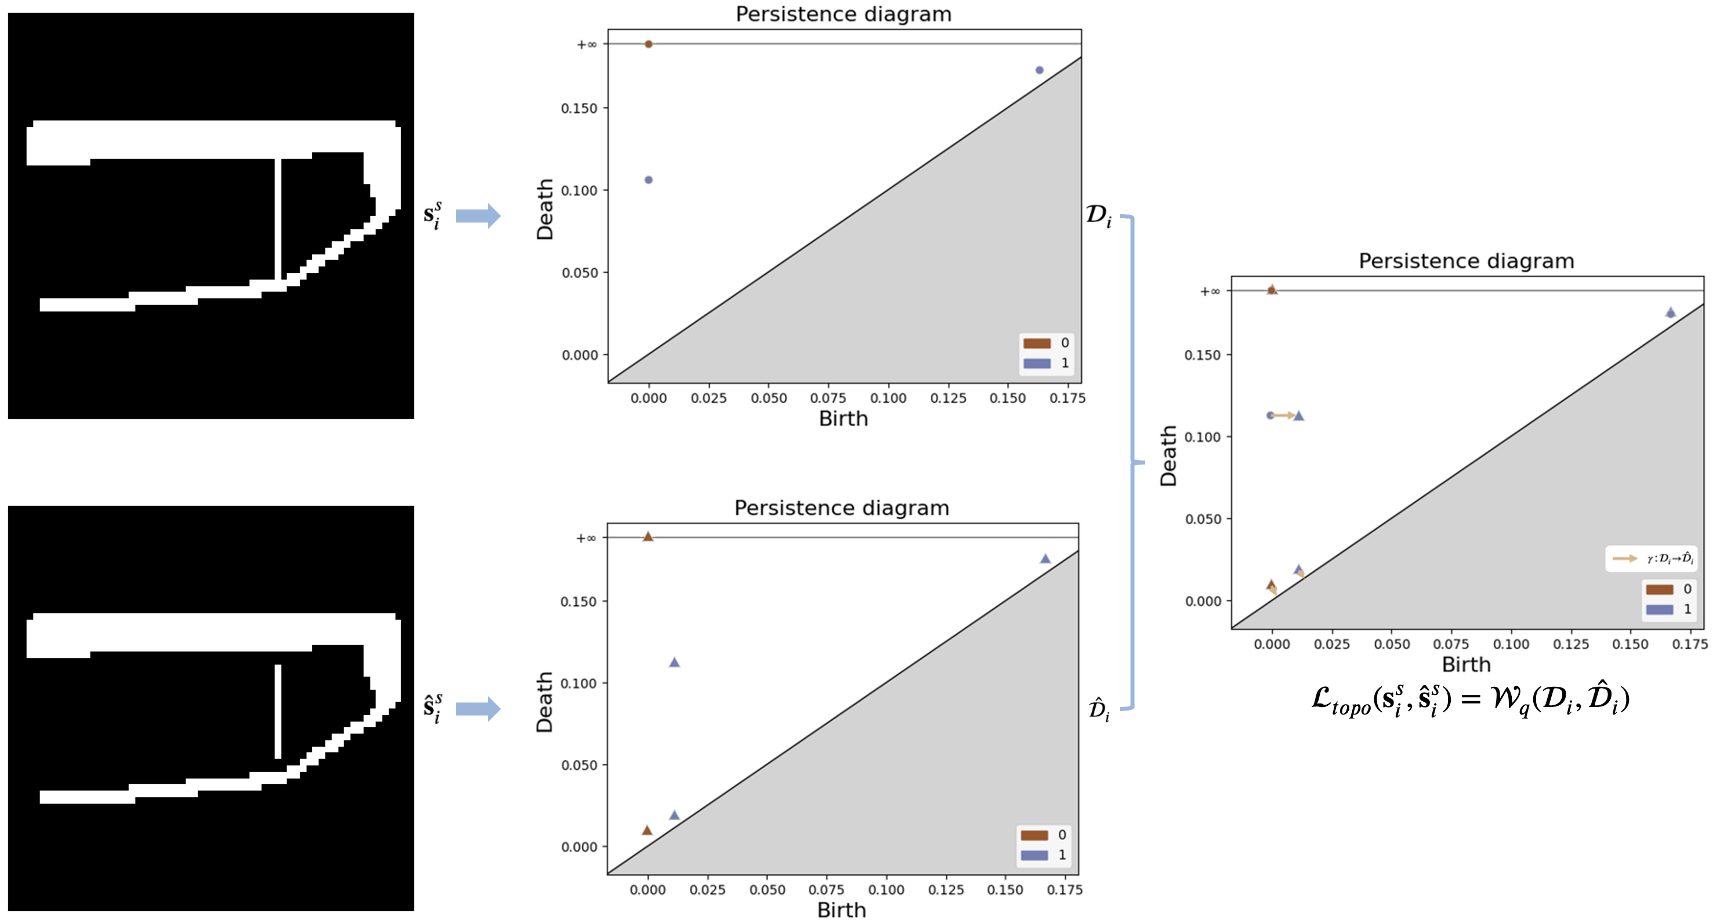
\includegraphics[width=0.9\linewidth]{./figures/TONIR/topo_illu.png}
    \caption{拓扑损失 $\mathcal{L}_{topo}$的说明}
    \label{fig:topo_loss_illu}
\end{figure}

为了获得结构$s$的可微拓扑特征,采用持久同调分析来导出其对应的持久图$\mathcal{D}$。如图~\ref{fig:topo_loss_illu}所示,将拓扑损失$\mathcal{L}_{topo}$定义为从GT和网络预测结构中获得的持久图$\mathcal{D}_i$和$\hat{\mathcal{D}}_i$之间的Wasserstein距离:
\begin{equation}
    \label{eq:topo-loss}
    \mathcal{L}_{topo}(\mathbf{s}_i^s, \hat{\mathbf{s}}^s_i)=\mathcal{W}_q(\mathcal{D}_i,\hat{\mathcal{D}}_i)=\left(\inf_{\gamma:\mathcal{D}_i\rightarrow\hat{\mathcal{D}}_i}\sum_{p\in\mathcal{D}_i}||p,\gamma(p)||^q\right)^{1/q},
\end{equation}
其中,$||\cdot||$是$L_2$范数,$\gamma$是$\mathcal{D}_i$和$\hat{\mathcal{D}}i$之间的双射,$q$是控制拓扑损失敏感度的超参数。在实验中,设定$q=2$。使用\textit{GUDHI}库~\cite{maria2014gudhi}计算拓扑损失。为了提高效率,采用了并行处理进行加速。如图~\ref{fig:loss_compare}所示,与几何损失相比,拓扑损失在捕捉结构缺陷和断裂方面更为有效。结构(a)是一个单连通($\beta_0=1$)且有一个孔($\beta_1=1$)的结构。与结构(a)相比,结构(b)由于缺少一个实心元素而断裂,导致孔消失($\beta_1=0$),但保持单连通组件($\beta_0=1$)。尽管结构特征发生了显著变化(高结构顺应性误差$\mathcal{E}{comp}$),缺少一个元素仍然导致低几何损失,而拓扑损失则表现出显著响应。由于缺少两个实心元素,结构(c)由两个断开的组件组成($\beta_0=2$)。同样,拓扑损失比相对较低的几何损失表现出更大的响应。为比较,设置了结构(d),其增加了一个实心元素,其拓扑特征与结构(a)保持一致。对于结构(d),几何损失、拓扑损失和顺应性误差都保持在相对较低的水平。因此,采用以下重构损失来训练深度神经网络,使网络能够更准确地重构结构,
\begin{equation}
    \label{eq:total-loss}
    \mathcal{L}_{recon}(\mathbf{s}_i^s, \hat{\mathbf{s}}^s_i)=\lambda_1\mathcal{L}_{geo}(\mathbf{s}_i^s, \hat{\mathbf{s}}^s_i)+\lambda_2\mathcal{L}_{topo}(\mathbf{s}_i^s, \hat{\mathbf{s}}^s_i),
\end{equation}
在实验中,设定权重$\lambda_1=0.7, \lambda_2=0.3$。拓扑损失的应用在某种程度上确保了输出结构的完整性。
\begin{figure}[htbp]
    \centering
    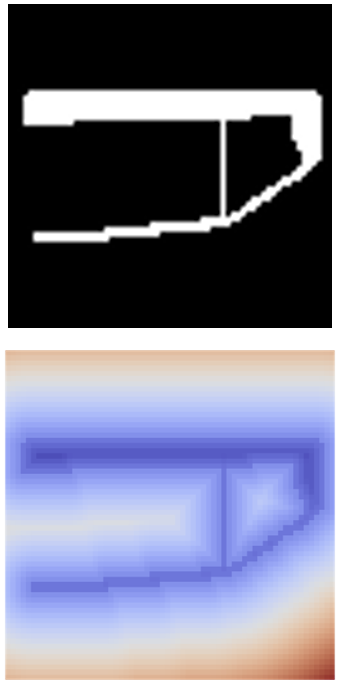
\includegraphics[width=0.2\textwidth]{./figures/TONIR/topo-a.png}
    \hspace{0.1cm}
    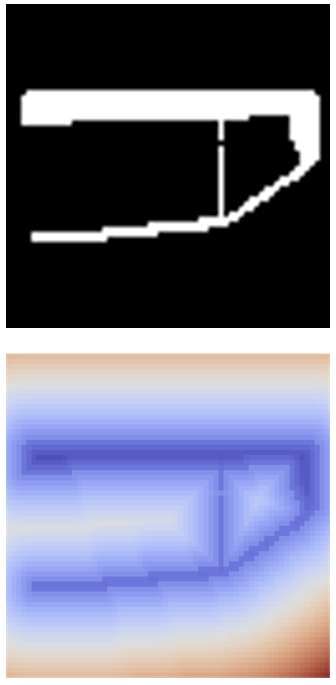
\includegraphics[width=0.2\textwidth]{./figures/TONIR/topo-b.png}
    \hspace{0.1cm}
    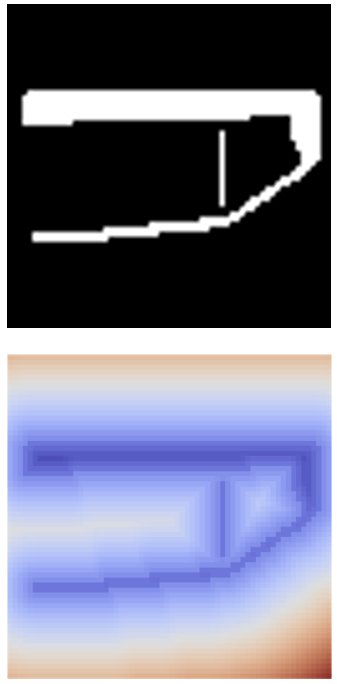
\includegraphics[width=0.2\textwidth]{./figures/TONIR/topo-c.png}
    \hspace{0.1cm}
    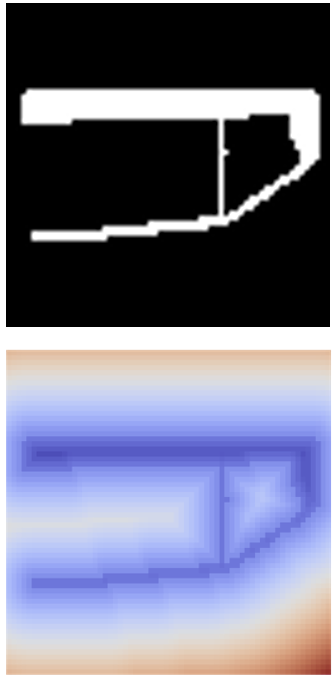
\includegraphics[width=0.2\textwidth]{./figures/TONIR/topo-d.png}
    \\
    \makebox[0.2\textwidth]{(a)}
    \hspace{0.1cm}
    \makebox[0.2\textwidth]{(b)}
    \hspace{0.1cm}
    \makebox[0.2\textwidth]{(c)}
    \hspace{0.1cm}
    \makebox[0.2\textwidth]{(d)}
    \\
    \vspace{0.2cm}
    \renewcommand{\arraystretch}{1.2}
    \begin{tabular}{c|c|c|c|c}
        \hline
        \textbf{指标}                     & \textbf{结构 a} & \textbf{结构 b} & \textbf{结构 c} & \textbf{结构 d} \\
        \hline
        $\mathcal{L}_{geo}$ (\textit{vs. a})  & 0                    & 0.00024              & 0.00098              & 0.00024              \\
        \hline
        $\beta_0$                             & 1                    & 1                    & 2                    & 1                    \\
        \hline
        $\beta_1$                             & 1                    & 0                    & 0                    & 1                    \\
        \hline
        $\mathcal{L}_{topo} (\textit{vs. a})$ & 0                    & 0.03125              & 0.03886              & 0.00937              \\
        \hline
        $\mathcal{E}_{comp} (\textit{vs. a})$ & -                    & 21.6\%               & 69.7\%               & 0.5\%                \\
        \hline
    \end{tabular}
    \caption{几何损失和拓扑损失的比较}
    \label{fig:loss_compare}
\end{figure}

除了重构损失外,VAE还需要KL散度损失来约束学习到的潜在空间分布,使其匹配预定义的先验分布~\cite{kingma2019introduction},这鼓励学习到的分布与先验分布相匹配,促进模型捕捉数据的基本特征。KL散度损失定义为:
\begin{equation}
    \mathcal{L}_{\text{KL}} = -\frac{1}{2} \sum_{i=1}^{N}(1 + \log(\sigma_i^2) - \mu_i^2 - \sigma_i^2)
\end{equation}
其中, $\mu_i$ 和$\sigma_i$ 分别表示第i个数据样本的学习潜在分布的均值和标准差,N是数据样本的总数。最小化KL散度损失鼓励潜在空间接近均值为零、方差为一的多元高斯分布,从而确保更好的样本生成和潜在空间插值特性。因此,使用下面总损失来训练IF-TONIR,
\begin{equation}
    \mathcal{L}_{total}=\mathcal{L}_{recon}+\mathcal{L}_{KL}
\end{equation}

\subsubsection{评估指标}
除了上述损失函数外,还使用重建准确性和物理准确性指标来评估IF-TONIR的性能。为了评估网络在结构重构方面的准确性,使用交并比(IoU)指标来量化GT结构与网络输出之间的差异,该指标常用于目标检测~\cite{IoU2019},
\begin{equation}
    \mathcal{E}^{IoU}_i=\frac{||~\Omega_{\hat{\mathbf{s}}^s_i} \cap \Omega_{\mathbf{s}^s_i}~||}{||~\Omega_{\hat{\mathbf{s}}^s_i} \cup \Omega_{\mathbf{s}^s_i}~||},
\end{equation}
其中,$\Omega_{\hat{\mathbf{s}}^s_i}$和$\Omega_{\mathbf{s}^s_i}$分别是被$\hat{\mathbf{s}}^s_i\leq 0$和$\mathbf{s}^s_i\leq 0$占据的区域。$||\cdot||$表示该区域的面积。

为了评估原始优化问题的目标和体积约束的有效性,进一步分析了相对体积和结构柔度的误差,
\begin{equation}
    \mathcal{E}^{vol}_i=\frac{|V(\hat{\mathbf{s}}^s_i)-V(\mathbf{s}^s_i)|}{V(\mathbf{s}^s_i)},
\end{equation}
\begin{equation}
    \mathcal{E}^{comp}_i=\frac{|C(\hat{\mathbf{s}}^s_i)-C(\mathbf{s}^s_i)|}{C(\mathbf{s}^s_i)}
\end{equation}
其中,$V(\mathbf{s}^s_i)=\int_{\Omega_{\mathbf{s}^s_i}}1\mathrm{d}A$,$C(\mathbf{s}^s_i)$在公式~\eqref{eq:opti_problem}中定义。

\subsection{训练和生成}
IF-TONIR算法表明,一旦神经网络经过充分训练并收敛,可以通过无迭代方法直接生成在体积约束下具有低顺应性的最优结构。算法~\ref{alg:algorithm1}中概述了IF-TONIR的训练过程。基于VAE网络,将优化结构的SDF嵌入低维潜在空间。通过从学习到的潜在空间中采样,可以生成新的结构。为了指导生成过程,将设计域形状、载荷和位移约束作为属性附加到空间坐标上,并结合从物理网络获得的条件信息。然后,使用训练好的解码器获得优化的结构。详细的生成过程如算法~\ref{alg:algorithm2}所示。
\begin{algorithm}[htbp]
    \caption{IF-TONIR 的训练}
    \label{alg:algorithm1}
    \begin{algorithmic}[1]
        \REQUIRE 结构的 GT SDFs: $\{\mathbf{s}^s_i\}_{i=1}^{N}$; 设计域: $\{\mathbf{s}^d_i\}_{i=1}^{N}$; 物理场: $\{\mathbf{s}^{phy}_i\}_{i=1}^{N}$; 体积约束: $\{v_i\}_{i=1}^N$; 采样点: $\{\mathbf{p}_k=(x_k, y_k)\}_{k=1}^M$
        \ENSURE 最优网络参数 $\Theta^*=\{\Theta^*_{vae}, \Theta^*_{phy}\}$
        \STATE 初始化网络 $\Phi^{E}_{vae}, \Phi^{D}_{vae}, \Phi_{phy}, \lambda_1, \lambda_2$
        \WHILE{未收敛}
            \STATE 将数据集划分为 $M$ 个批次 $\{\mathcal{T}_i\}_{i=1}^M$
            \FORALL{批次 $\mathcal{T}_i$}
                \STATE 初始化 $\mathcal{L}^i_{geo}=0, \mathcal{L}^i_{topo}=0$
                \FORALL{批次中的样本 $\mathbf{s}_j$}
                    \STATE 计算结构潜在编码: $\mathbf{z}_j=\Phi^E_{vae}(\mathbf{s}^s_j)$
                    \STATE 计算点属性向量: $\mathbf{c}^{prop}_{k}=[\gamma(x_k),\gamma(y_k),\gamma(\mathbf{s}^{d}_i),\gamma(v_i)]$
                    \STATE 计算条件编码: $\mathbf{c}^{phy}_j=\Phi_{phy}(\mathbf{s}^{phy}_j)$
                    \STATE 连接潜在编码: $\mathbf{l}_j=[\mathbf{z}_j, \mathbf{c}^{prop}_{k}, \mathbf{c}^{phy}_j]$
                    \STATE 计算重构的 SDF: $\hat{\mathbf{s}}^s_j=\Phi^D_{vae}(\mathbf{l}_j)$
                    \STATE 评估几何损失: $\mathcal{L}^i_{geo}=\mathcal{L}^i_{geo}+(\mathcal{L}_{clamp}(\hat{\mathbf{s}}_j^s, \mathbf{s}_j^s)+0.1*\mathcal{L}_{mse}(\hat{\mathbf{s}}_j^s, \mathbf{s}_j^s))$
                    \STATE 通过持久同调计算 PDs: $\mathcal{D}_j, \hat{\mathcal{D}}_j$
                    \STATE 评估拓扑损失: $\mathcal{L}^i_{topo}=\mathcal{L}^i_{topo}+\mathcal{W}_q(\hat{\mathcal{D}}_j, \mathcal{D}_j)$
                    \STATE 评估重构损失: $\mathcal{L}^i_{recon}=\lambda_1\mathcal{L}^i_{geo}+\lambda_2\mathcal{L}^i_{topo}$
                \ENDFOR
                \STATE 评估总损失函数: $\mathcal{L}^i_{total}= \mathcal{L}^i_{recon}+\mathcal{L}_{KL}$
                \STATE 通过 $\frac{\partial \mathcal{L}^i_{total}}{\partial \Theta}$ 更新 $\Theta$
            \ENDFOR
        \ENDWHILE
    \end{algorithmic}
\end{algorithm}


\begin{algorithm}[htbp]
    \caption{通过 IF-TONIR 生成最优结构}
    \label{alg:algorithm2}
    \begin{algorithmic}[1]
        \REQUIRE 设计域: $\mathbf{s}^d$; 边界条件: 载荷和位移约束; 体积约束: $v$; 设计域内的采样点: $\{\mathbf{p}_k\}_{k=1}^M$; 最优网络参数: $\Theta^*=\{\Theta^*_{vae}, \Theta^*_{phy}\}$
        \ENSURE 在给定体积约束 $v$ 下具有最小柔度的最优结构 $\mathbf{s}^*$
        \STATE \textbf{步骤 1:} 从标准高斯分布中采样形状潜在编码 $\mathbf{z}\sim\mathcal{N}(0, 1)$
        \STATE \textbf{步骤 2:} 计算点属性向量: $\mathbf{c}^{prop}_{k}=[\gamma(x_k),\gamma(y_k),\gamma(\mathbf{s}^{d}),\gamma(v)]$
        \STATE \textbf{步骤 3:} 根据边界条件计算物理场 $\mathbf{s}^{phy}$
        \STATE \textbf{步骤 4:} 计算物理潜在编码: $\mathbf{c}^{phy}=\Phi_{phy}(\mathbf{s}^{phy}; \Theta^*_{phy})$
        \STATE \textbf{步骤 5:} 计算体积约束编码: $\gamma(v)$
        \STATE \textbf{步骤 6:} 连接潜在编码: $\mathbf{l}=[\mathbf{z}, \mathbf{c}^{prop}_k, \mathbf{c}^{phy}]$
        \STATE \textbf{步骤 7:} 生成最优结构的SDF: $\mathbf{s}_s^*=\Phi^D_{vae}(\mathbf{l}; \Theta^*_{vae})$
        \STATE \textbf{步骤 8:} 从SDF中提取结构: $\mathbf{s}^*$
    \end{algorithmic}
\end{algorithm}

\section{实验和分析}

\subsection{超参数设置和收敛性}
本算法所用的训练数据集包含 26796 个样本,涵盖了 图~\ref{fig:datasets} 所示的设计领域。对于每个训练 epoch,随机选择 21437 个样本 (占 80\%) 用于训练,5359 个样本 (占 20\%) 用于验证。模型在包含 924 个样本的测试数据集上进行评估,这些样本来自未见过的设计领域。

模型根据 算法~\ref{alg:algorithm1} 在配备 Nvidia A40 GPU 的机器上进行训练,使用 Adam 优化器,初始学习率为 0.001,每 20 个 epoch 将学习率减少 0.5 倍。在训练过程中,将结构刚度作为损失函数或准确性指标是非常耗时的。尽管 TopoDiff~\cite{maze2022} 提出了一个回归模型来预测生成结构的刚度,但需要额外的数据准备和网络训练。因此,使用 IoU 指标来监控训练过程,将来会将物理量监督纳入考虑。 图~\ref{fig:training} 展示了训练过程中损失和 IoU 准确性的稳定收敛。可以观察到,随着训练的进行,生成的结构逐渐变得更加合理和稳健。大约需要 150 个 epoch 才能得到 IoU 准确性约为 94\% 的预测结果。
\begin{figure}[htbp]
    \centering
    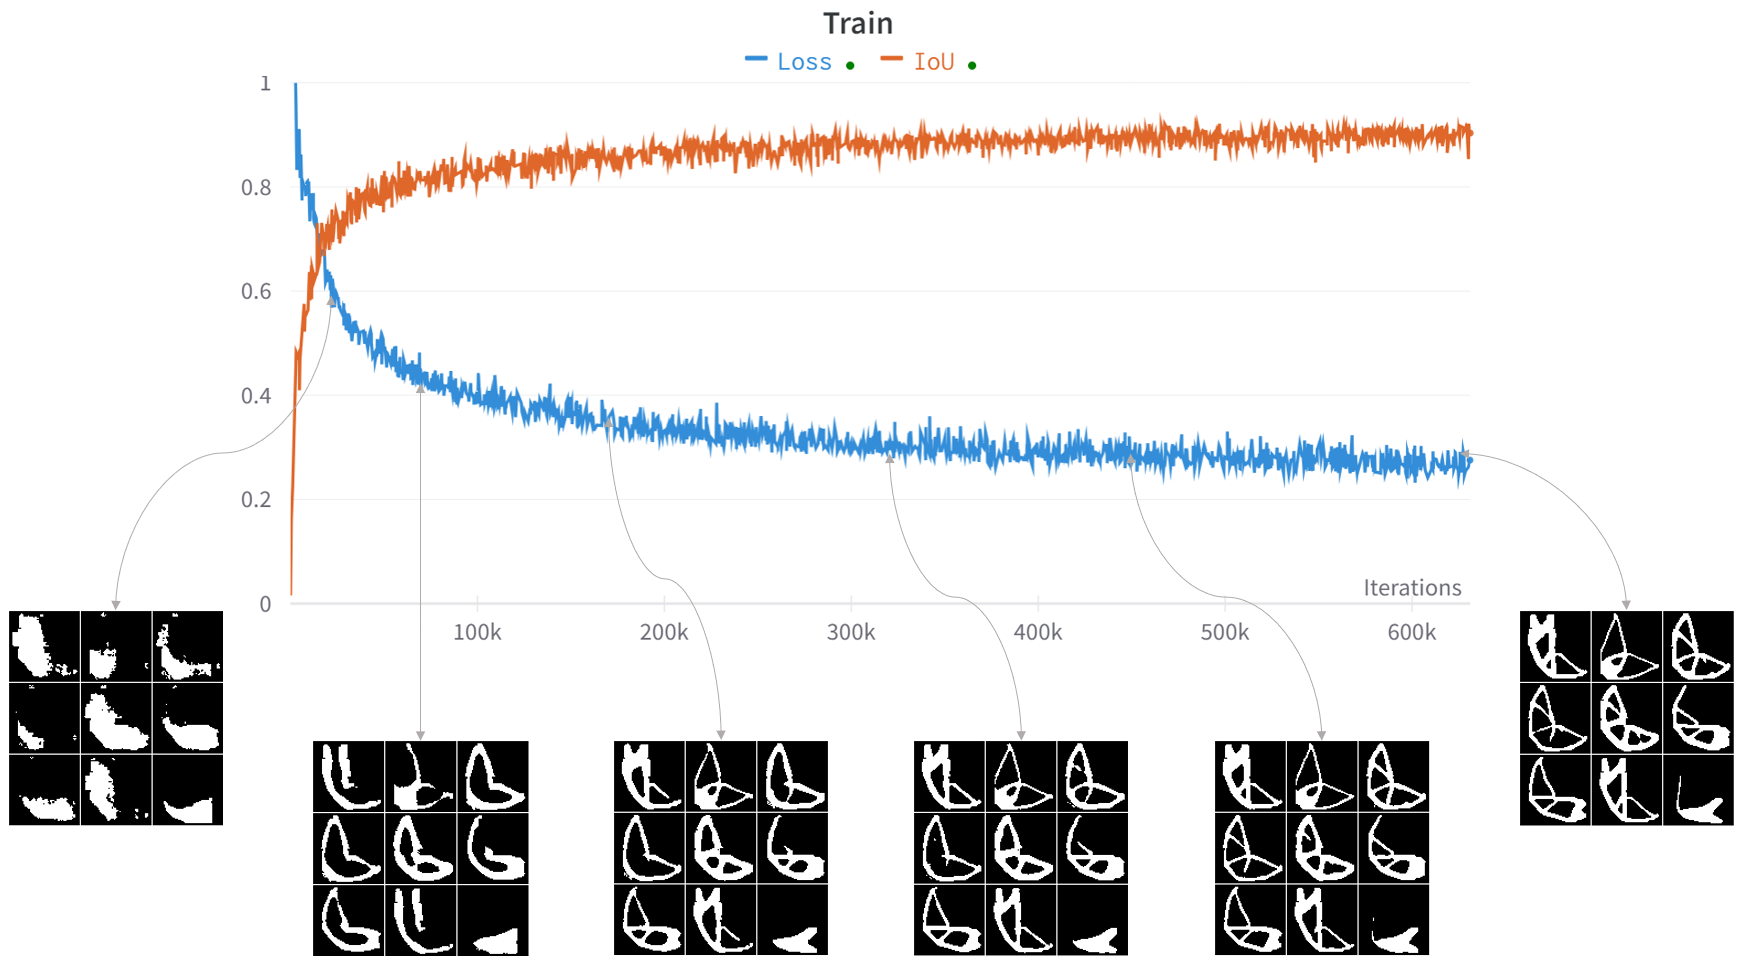
\includegraphics[width=0.85\textwidth]{./figures/TONIR/fig-convergence.png}
    \caption{IF-TONIR的训练过程}
    \label{fig:training}
\end{figure}

\subsection{性能评估}
完成训练后,评估生成结构在结构刚度和体积方面的准确性。如 图~\ref{fig:eval-train} 所示,IF-TONIR 成功预测出了与训练数据集中 GT 样本非常相似的结构,它准确地识别了设计域的形状以及施加载荷的位置。在整个训练数据集上,IF-TONIR 的平均刚度误差为 6.90\%,平均体积误差为 1.32\%。为验证 IF-TONIR 的有效性,在测试数据集上评估其性能,如 图~\ref{fig:eval-test} 所示。测试数据集的平均刚度误差为 54.2\%,平均体积误差为 4.02\%。值得注意的是,测试数据集包含了两种训练过程中未观察到的设计域形状。因此,测试数据集中的边界条件位置与训练数据集完全不同。据悉,该算法是首个将设计域形状作为泛化能力一部分的算法。
\begin{figure}[htbp]
    \centering
    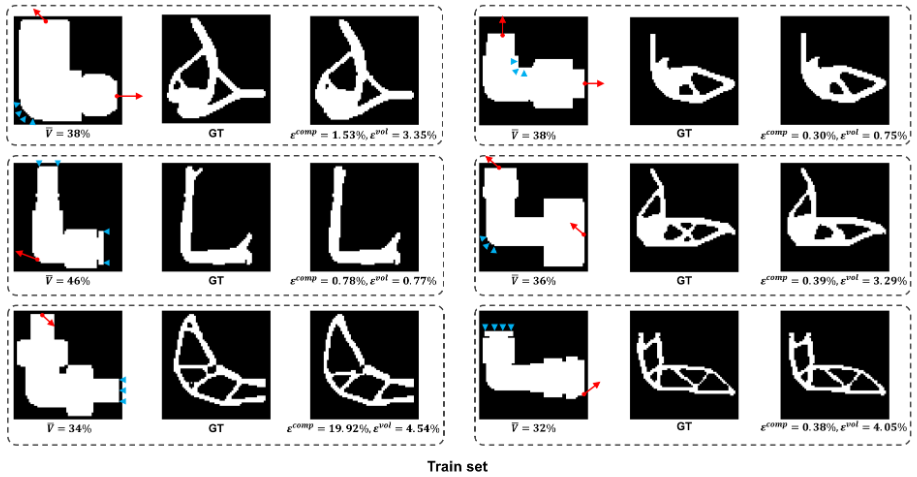
\includegraphics[width=0.95\textwidth]{./figures/TONIR/results-train.png}
    \caption{训练数据集上的测试结果}
    \label{fig:eval-train}
\end{figure}
\begin{figure}[htbp]
    \centering
    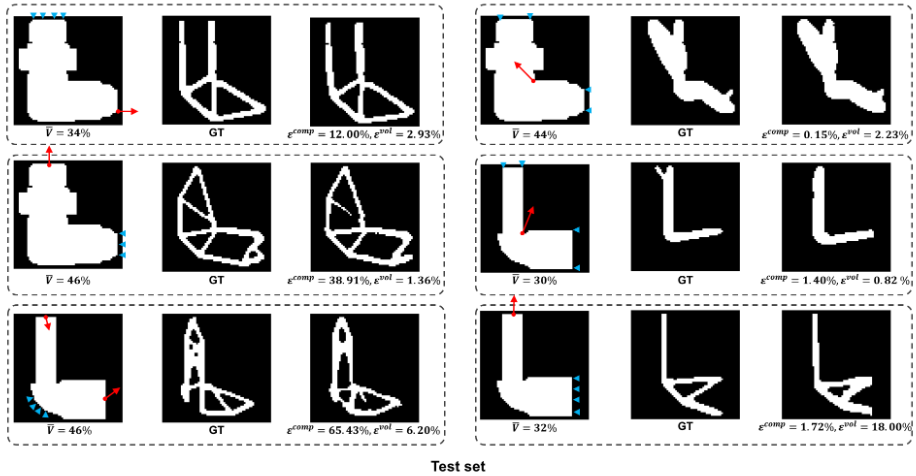
\includegraphics[width=0.95\textwidth]{./figures/TONIR/results-test.png}
    \caption{测试数据集上的测试结果}
    \label{fig:eval-test}
\end{figure}


\subsection{消融实验}
\paragraph{拓扑损失。}
结构不连续性常会导致不稳定或高刚度,图~\ref{fig:topo-comparison} 说明了拓扑损失在改善生成结构的结构连续性方面的有效性。由于采用结构的 SDFs 作为计算持续同调的过滤值,所得到的 PD 可以有效捕捉数据的几何和拓扑特征。连续的过滤值场使训练过程更加稳定,从而使网络生成的结构能够与 GT 样本非常相似。
\begin{figure}[htbp]
    \centering
    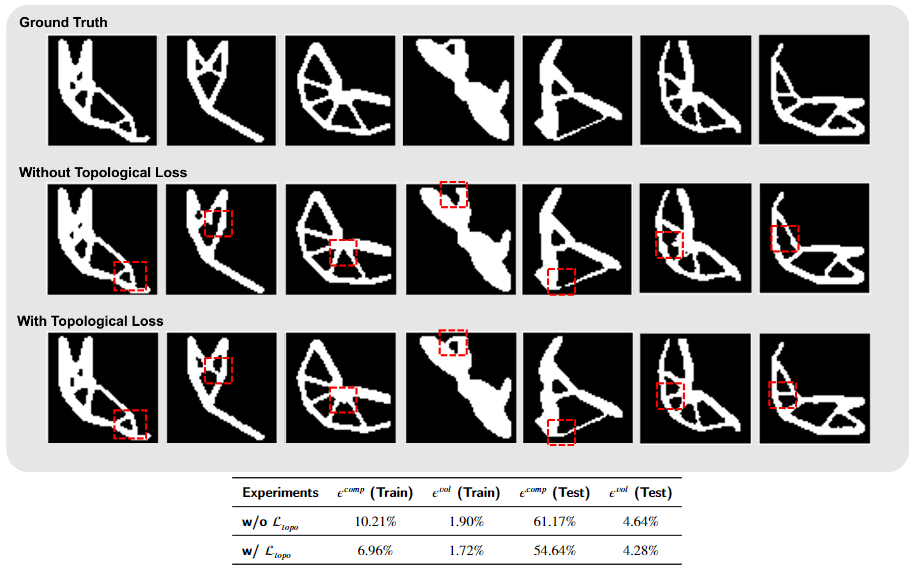
\includegraphics[width=0.95\textwidth]{./figures/TONIR/abla-topo.png}
    \caption{拓扑损失的消融实验结果}
    \label{fig:topo-comparison}
\end{figure}
\begin{figure}[htbp]
    \centering
    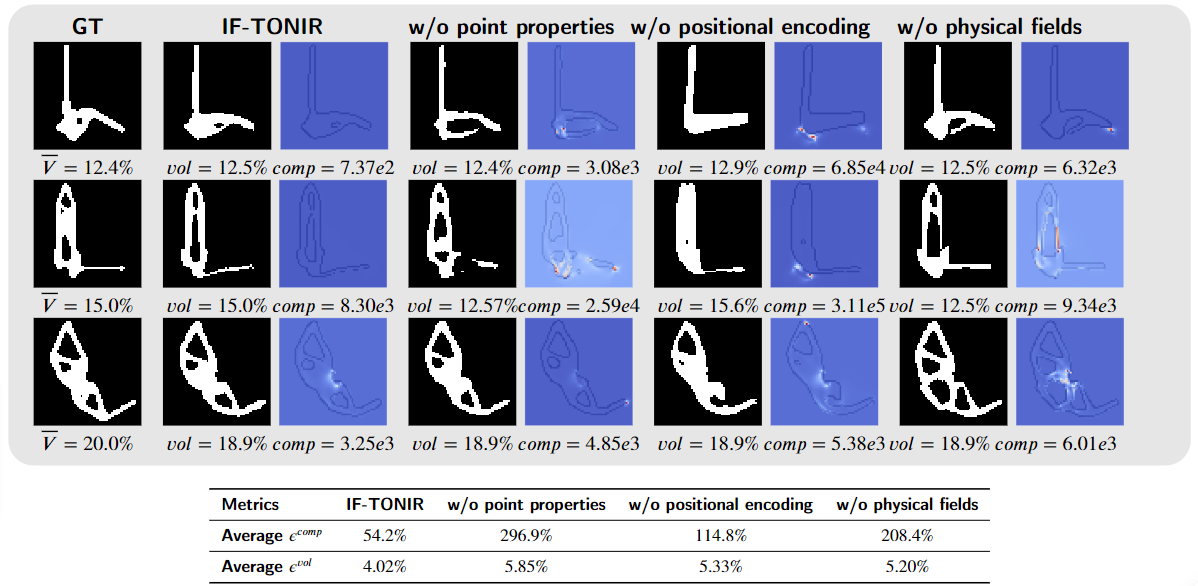
\includegraphics[width=0.95\textwidth]{./figures/TONIR/abla-pp.png}
    \caption{点属性和物理场的消融实验结果}
    \label{fig:ablation}
\end{figure}

\paragraph{点属性。}
确定特定点的 SDF 值时,将设计形状信息和体积约束作为点属性,与坐标一起使用。这些点属性还可包括载荷位置和位移约束。本方法不同于之前的方法在于将体积约束作为解码器中点属性的一部分,而非复制以匹配输入张量大小。未使用点属性的对照实验表明其关键作用,如 图\ref{fig:ablation} 所示。通过对其值应用高频变换(如公式~\eqref{eq:pe}中的位置编码)增强算法中点属性的影响。消融实验验证位置编码的重要性,结果表明位置编码层有助于网络预测更准确的体积和力的施加位置。使用位置编码的平均刚度几乎只有未使用位置编码的六分之一,表明结构强度更高,如 图~\ref{fig:ablation} 中的几个示例所示。

\paragraph{物理场。}
之前的工作已证实,原始设计域上的物理场信息在预测最优结构方面发挥着积极作用。为说明其对算法的重要性,如 图~\ref{fig:ablation} 所示,从物理信息中删除应力和应变能场后出现的不利影响。

\subsection{比较实验}
本节对 IF-TONIR 与其他生成模型(TopologyGAN~\cite{topologygan2021}和 TopoDiff~\cite{maze2022})进行了比较分析。值得注意的是,这些先前的工作未考虑设计域形状。为确保公平比较,这里在 TopoDiff 提供的相同数据集上评估了这三个模型。由于该数据集中的结构是在固定的规则设计域上生成的,只需从 IF-TONIR 中删除与域相关的信息,即可在提供的数据集上进行训练和评估。图~\ref{fig:comparison} 展示了 IF-TONIR、TopologyGAN 和 TopoDiff 之间的比较结果。
\begin{figure}
    \centering
    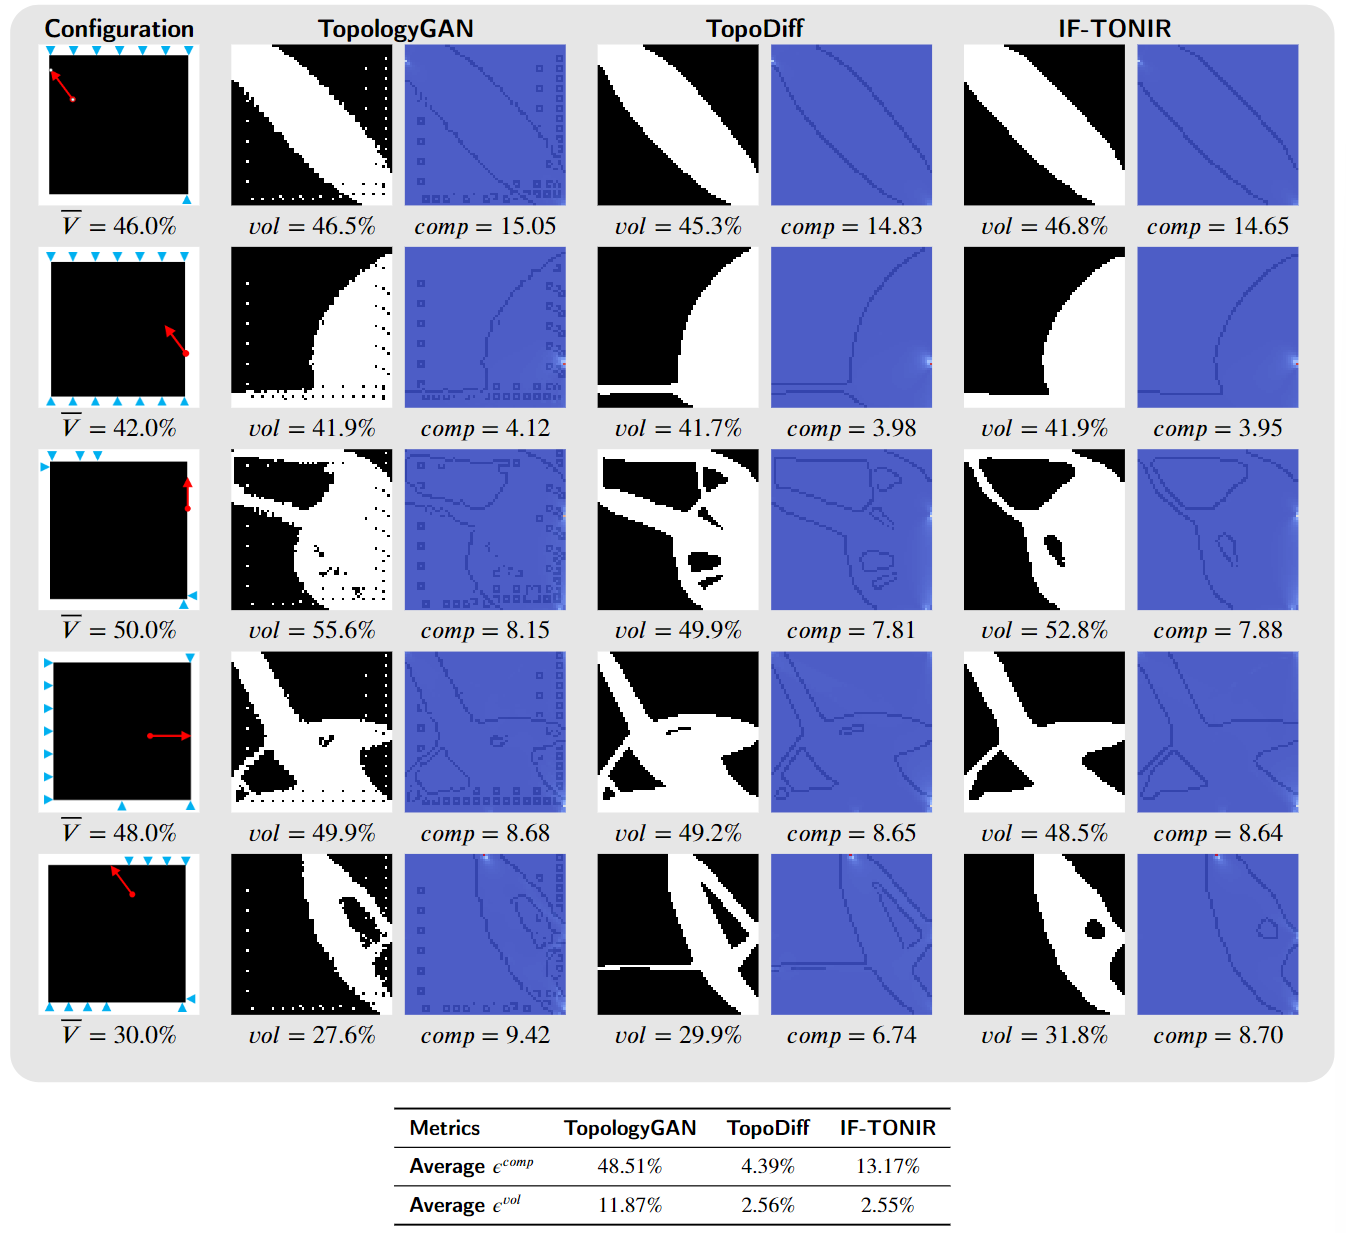
\includegraphics[width=0.95\linewidth]{./figures/TONIR/results-comparison.png}
    \caption{IF-TONIR与其他生成模型的比较}
    \label{fig:comparison}
\end{figure}

作为最受欢迎的生成模型之一,扩散模型已被证明在捕捉图像或形状生成中的细节方面具有更强的能力,如 图~\ref{fig:comparison} 所示。此外,TopoDiff 框架结合了三个子网络来增强生成结构的强度和连续性。因此,从图~\ref{fig:comparison} 中的表格可以观察到,TopoDiff 目前取得了最佳性能。但需要注意的是,TopoDiff 在所比较的模型中具有最高的复杂度,生成结构需要更长的推理时间,需要 21.59 秒,而 IF-TONIR 只需 0.09 秒(在 CPU 上)。此外,将扩散模型扩展到 3D 域存在计算效率和内存利用方面的挑战。相比之下,IF-TONIR 在更轻的网络架构下取得了优于 GAN 模型的结果。众所周知,训练 GAN 模型是一项艰难的任务。该框架还展示了跨不同形状设计域进行推广的能力,这在之前的工作中未被考虑。然而,与其他 VAE 模型类似,IF-TONIR 在生成具有细节的结构方面仍有局限性,这是未来工作的重点领域。

TopologyGAN 和 TopoDiff 要求输入和输出分辨率保持一致,这在生成高分辨率结构时会带来挑战。这需要准备一个新的高分辨率样本数据集,或采用超分辨率等技术。然而,由于 IF-TONIR 使用了隐式神经表示,可以以任意所需的分辨率获得结构。如图~\ref{fig:resolution} 所示,训练好的网络允许通过增加设计域内的采样点数来生成更高分辨率的结构。值得注意的是,IF-TONIR 可以在 CPU 上以约 10 秒的时间生成 1024 分辨率的结构。与传统的 SIMP 方法相比,该方法消除了获得平滑和连续结构表示的后处理需求。需要澄清的是,这里的分辨率指最终结构表示的分辨率,而不是结构特征的分辨率,提高结构表示的分辨率并不会增加更多的结构细节。
\begin{figure}[!h]
    \centering
    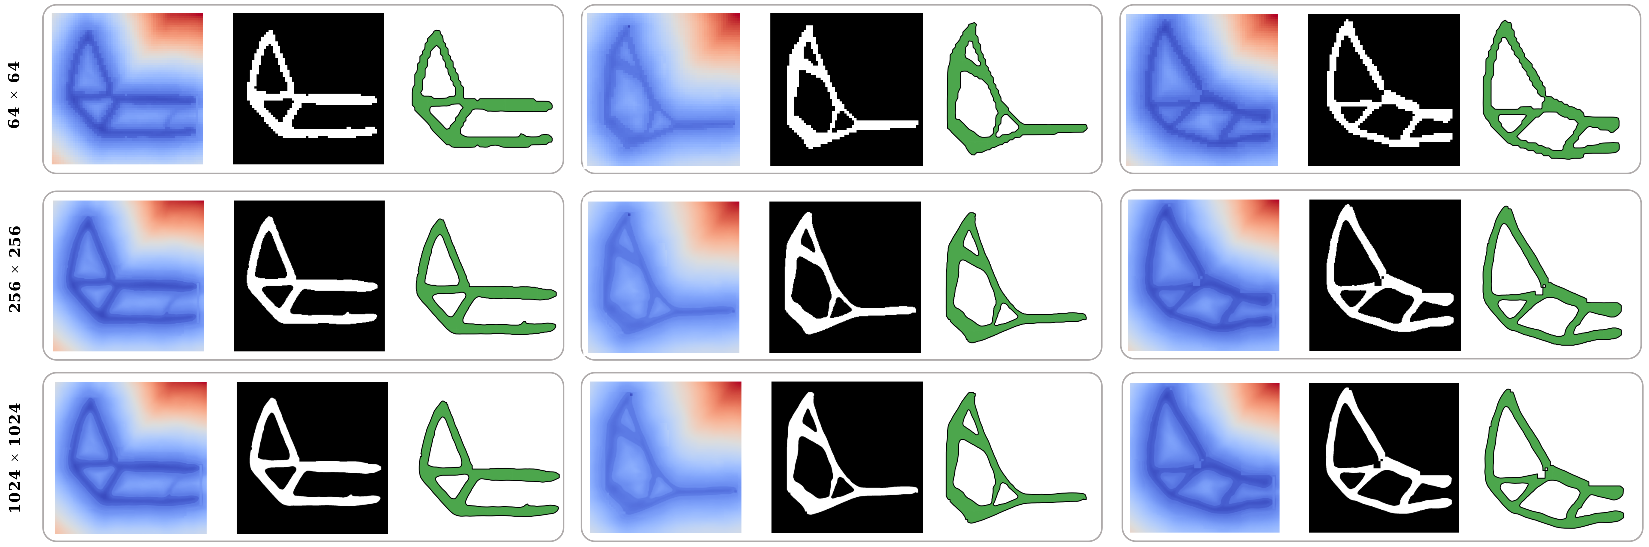
\includegraphics[width=0.9\textwidth]{./figures/TONIR/fig-resolution.png}
    \caption{IF-TONIR可以生成任意分辨率下的结构}
    \label{fig:resolution}
\end{figure}

\section{本章小结}
本文提出了 IF-TONIR,一种全新的无迭代拓扑优化方法。该算法利用隐式神经表示直接从给定条件和问题配置中生成优化结构。通过在测试数据集上的实验,IF-TONIR 展示了在生成各种类似形状设计域的优化结构方面的有效性,实现了较低的结构柔度。据悉,这是首个将拓扑优化过程推广到不同设计域形状的端到端工作。利用隐式神经表示将网络与空间网格解耦,理论上可以以任意所需的分辨率生成结构。此外,这种平滑紧凑的表示方法有效避免了棋盘现象。综上,本章算法在提高拓扑优化效率和应用性上主要有以下贡献:
\begin{itemize}
    \item 提出了一种全新的无迭代拓扑优化方法,可以直接从各种设计域形状和边界条件中输出最优结构。
    \item 除了常用的几何损失外,还引入了基于持续同调的拓扑损失,以量化结构的连续性,有效检测和测量即使是微小的结构断开。
    \item IF-TONIR 生成了结构的紧凑平滑的隐式表示,将设计过程与空间网格分离,理论上可以以任意所需的分辨率生成结构。
\end{itemize}